\documentclass{article}
\usepackage{color}
\usepackage{tikz}
\usepackage{float}
\usepackage{tabularx}
\usepackage{amsmath}
\usepackage{amssymb}
\usepackage{listings}
\usepackage{enumitem}
\usepackage{syntax}
\usepackage{csquotes}
\usepackage[backend=biber]{biblatex}
\addbibresource{references.bib}

\usepackage{tikz}
\usetikzlibrary{automata,positioning}

\definecolor{dkgreen}{rgb}{0,0.6,0}
\definecolor{gray}{rgb}{0.5,0.5,0.5}
\definecolor{mauve}{rgb}{0.58,0,0.82}


\lstset{frame=tb,
  numbers=left,
  stepnumber=1,
  language=Java,
  aboveskip=3mm,
  belowskip=3mm,
  showstringspaces=false,
  columns=flexible,
  basicstyle={\small\ttfamily},
  numberstyle=\color{gray},
  keywordstyle=\color{blue},
  commentstyle=\color{dkgreen},
  stringstyle=\color{mauve},
  breaklines=true,
  breakatwhitespace=true,
  tabsize=2,
  moredelim=**[is][\color{red}]{@}{@},
}

\setlength{\grammarindent}{12em}

%\renewcommand{\lstlistingname}{Algorithm}
%\newcommand{\tablerow}[4]{ #1 & #2 & #3 & #4\\}
\newcommand{\n}[0]{\\[\baselineskip]}
%\newcommand{\qa}[2]{\textbf{Q:} #1 \\ \textbf{A:} #2}
%\newcommand{\argument}[4]{\textbf{#1:} #2 \\ \textbf{#3:} #4}

\title{CS4303 Particle Command Report}
\author{Sizhe Yuen}

\begin{document}

\maketitle

\section{Introduction}
In this practical we were tasked to implement the video game \textit{Particle Command}, which is a variant on missile command where the particles are blasted away from the explosion rather than being destroyed. In my game, I have implemented all the features in the practical specifications as well as some additional features.
\n
TODO RUN INSTRUCTIONS

\section{Game features}

\subsection{Basic}
\subsubsection*{Meteors}
The particles falling are implemented in the \texttt{Meteor} class. They spawn from a random location at the top of the screen and have a random initial velocity. This initial random velocity goes from \texttt{-2f} to \texttt{2f} in the x direction and from \texttt{0} to \texttt{3f} in the y direction. The random y velocity makes some particles come down faster than others to make the game a bit more interesting. They do not have a random negative y velocity because all particles not in the screen are destroyed. 

\subsubsection*{Cities}
There are five locations where the cities are placed on the ground of the play area. These are static and do not change. This was done for simplicity and a fair balance so there are not occasional games where the cities are very far away, making the game more difficult. 

\begin{figure}[H]
\centering
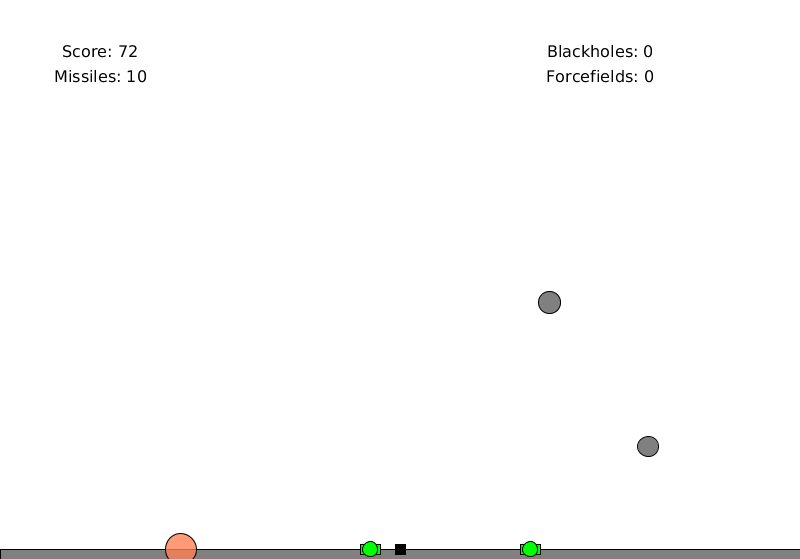
\includegraphics[width=1\textwidth, keepaspectratio]{imgs/Meteors.png}
\caption{Meteors falling from the sky. The one on the left has hit the ground and caused an explosion. Remaining cities can be seen in green.}
\end{figure}

\subsubsection*{Explosions}
All particles can create explosions when they are destroyed as it is an abstract method all \texttt{Particle} subclasses must implement. In my game, both the meteors and player missiles create explosions. The explosion radius is based off of the particle's initial radius, increasing with each time step until they've reach the end of their lifespan. Any particles caught in the blast radius are blown away with an \texttt{Explosive} force. 
\begin{figure}[H]
\centering
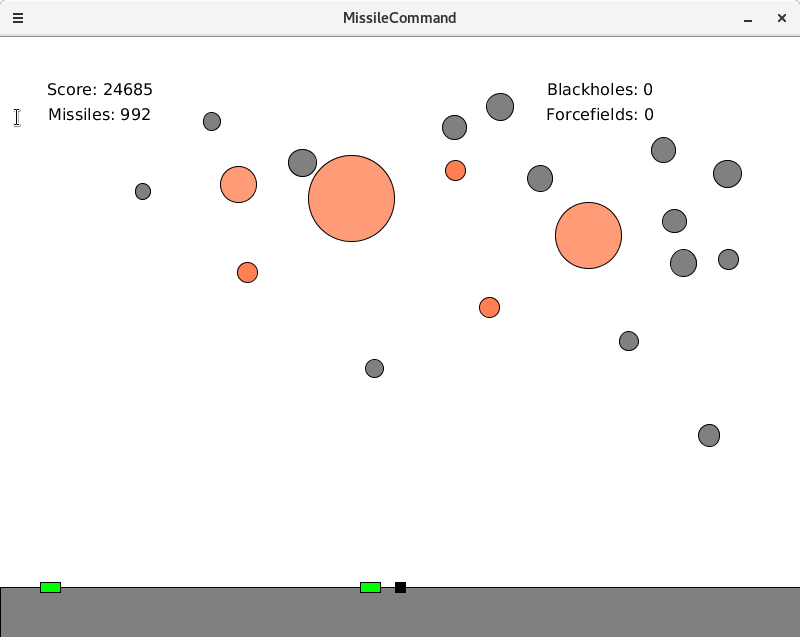
\includegraphics[width=1\textwidth, keepaspectratio]{imgs/NormalExplosion.png}
\caption{Normal explosions from player missiles.}
\end{figure}
\noindent
Initially both player missile explosions and meteor explosions can destroy cities. This was because they were the same piece of code and did not differentiate between them. However, I thought it was good to keep it like this because it prevents the player from just clicking missiles on top of their cities and deflecting all meteors. Since I have also implemented a shop, I have allowed players to purchase a permanent upgrade so missile explosions do not destroy the cities any more. The colour of the missiles and explosions also change to indicate this. 


\subsubsection*{Player missiles}
The player missiles fire from the center of the ground. Their velocity is normalised and not very fast so it takes a bit of planning to properly defend the cities that are further away. The missile explode either when they reach their destination - the position of the mouse cursor when the missile was fired - or when they collide with a meteor during their trajectory. 
\begin{figure}[H]
\centering
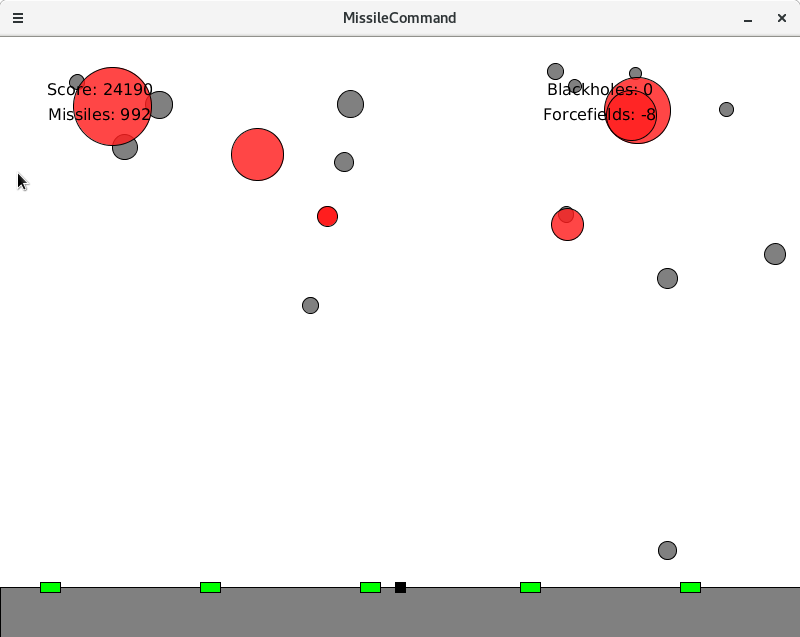
\includegraphics[width=1\textwidth, keepaspectratio]{imgs/UpgradedExplosion.png}
\caption{Upgraded explosions from player missiles. These do not destroy cities. The colour is different to indicate the change.}
\end{figure}

\subsubsection*{Waves}
The game is organised into waves. At the beginning of each wave, the number of missiles the player has is increased. Each wave has increasing difficulty as more meteors are spawned. Every few waves, the player is rewarded with a black hole or forcefield to help them survive. However, every few waves a bomber also comes which makes the game more difficult.
\begin{figure}[H]
\centering
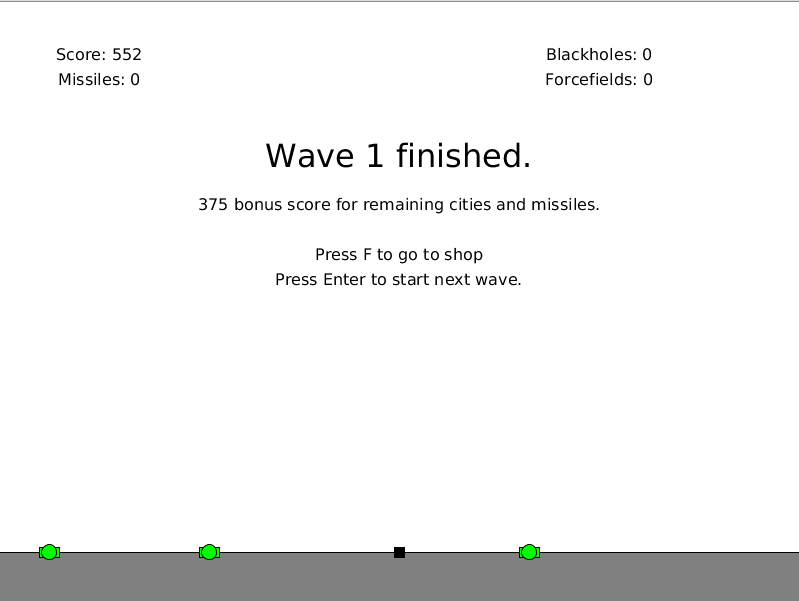
\includegraphics[width=1\textwidth, keepaspectratio]{imgs/WaveFinished.png}
\end{figure}


\subsection{Extension}

\subsubsection*{Split into child meteors}
To make the game more difficult, the extension for splitting meteors into child meteors is also implemented. Meteors that are larger than a certain radius have a chance to split into 2 or more child meteors. As the player goes into higher levels, the number of child meteors that spawn is increased. Meteors only begin to split at a certain level (\texttt{METEOR\_SPLIT\_STARTING\_LEVEL}) so the beginning of the game isn't too hard. 

\subsubsection*{Bombers}
In addition to splitting the meteors, bombers that drop "bombs" are also implemented in the game. These bombers fly across the screen and drop "bombs" that are much heavier than normal meteors. They are also given an initial downwards velocity to make them fly faster towards the player's cities.
\n
In the code, the bombs are implemented as meteors but drawn with a darker colour. This is because apart from flying faster to the ground they are the same as regular meteors. 

\subsubsection*{Black holes}
To add the force of gravitational attraction to the game, I added a special missile that player's can shoot which would create a black hole. The black holes apply gravitational attraction to all meteors on screen and because they are intentionally much heavier than the meteors, most will be sucked into the black hole and destroyed. Meteors that are further away may be affected less.
\begin{figure}[H]
\centering
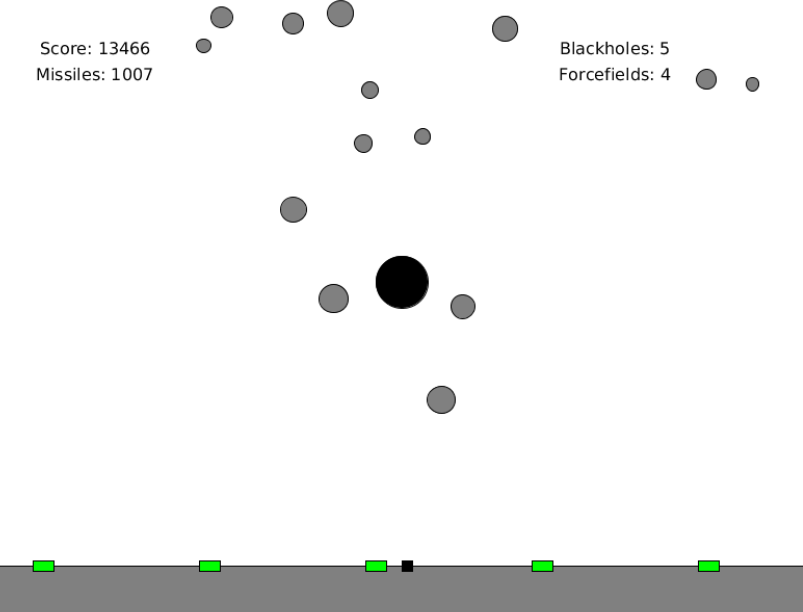
\includegraphics[width=1\textwidth]{imgs/Blackhole.png}
\end{figure}
The black holes only last for a short while before disappearing. This means that if a meteor was being accelerated towards it but did not get sucked in, it will no longer have a force applied to it, but it will retain its fast velocity, only being slowed by drag. This makes the use of black holes more strategic and a double edged sword if used improperly as the disappearing of one at the wrong time could cause a meteor to crash down really fast onto a city. Because of this danger, the black hole missiles will not create a black hole on impact, only when they reach their destination. Use right click instead of left click to shoot out a missile that creates a black hole.
 
\subsubsection*{Forcefield}
Unlike explosions, forcefield use a different kind of force to repel particles which makes them a more global and powerful tool to deflect meteors compared to missiles. Instead of applying an explosive force to knock the meteors away, forcefields use the opposite force of gravitational attraction. The meteors are repulsed away from the forcefield by multiplying the force of gravitational attraction by -1. 
\begin{figure}[H]
\centering
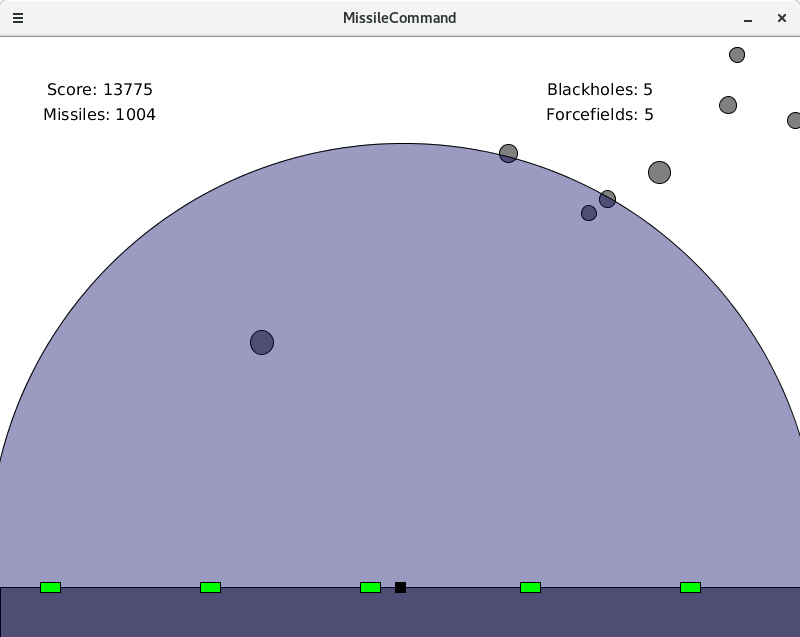
\includegraphics[width=1\textwidth]{imgs/Forcefield.png}
\end{figure}
\noindent
This also means that the display of the forcefield moving outwards does not properly reflect how it works as the radius does not affect how much the particles are pushed away by. However, it does show what the forcefield does in an easy way to understand. The button for using forcefields is the middle mouse button.

\subsubsection*{Shop}
To allow the player the ability to use more of these special particles, I have added a little shop screen for players to spend score to purchase extra black holes, forcefields and missiles. Because these cost score to buy, the player must choose between keeping their score high, or using it to ensure they don't lose in the next round. 
\begin{figure}[H]
\centering
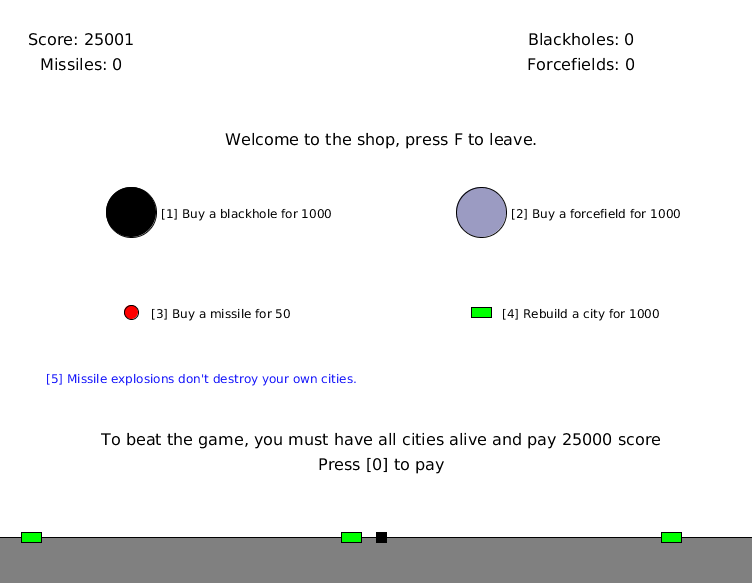
\includegraphics[width=1\textwidth, keepaspectratio]{imgs/Shop.png}
\end{figure}


\section{Design}

\subsection{Scoring system}
There are two components to the scoring system: during the wave and at the end of the wave. \n
During the wave, if a meteor hits the ground and explodes, it adds a bit of score. If the meteor is instead knocked away outside of the screen, more score is added. By having meteors give score regardless, it allows players who are not very skilled to still get score that they can use in the shop. 
\subsection{Increasing difficulty}
There are multiple things that I've done to increase the difficulty of the game. 
\begin{itemize}
\item Increase number of meteors every wave.
\item Bombers start to appear on the fifth wave and every fifth wave adds another bomber.
\item Meteors have increased mass which causes them to have a higher chance of splitting into smaller meteors.
\item Number of child meteors from a meteor splitting also increases 
\end{itemize}
\subsection{City arrangement}
The city arrangement is static and in evenly spread locations. This is so there aren't any balance issues with cities being too concentrated in certain locations. The number of cities can be changed and the game is able to place any number of them evenly. 
\begin{figure}[H]
\centering
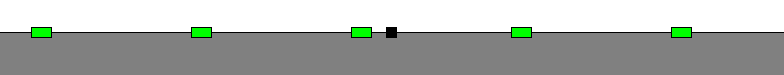
\includegraphics[width=1\textwidth, keepaspectratio]{imgs/FiveCities.png}
\caption{Five cities}
\end{figure}

\begin{figure}[H]
\centering
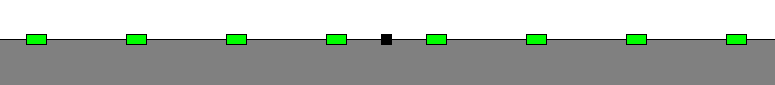
\includegraphics[width=1\textwidth, keepaspectratio]{imgs/EightCities.png}
\caption{Eight cities}
\end{figure}
\noindent

\section{Implementation}
\subsection{Particles}
Almost all the game objects inherit from the abstract \texttt{Particle} class. This class contains all the fields that game objects need like position, velocity and the force accumulator. The \texttt{Particle} super class also implements the \texttt{IDrawable} interface, which means all particle sub classes must include a display function.
\n
This design allows each class to define its own draw function and change it accordingly based on its properties. For example an explosion has increasing radius as it is drawn, or a missile should stop displaying after reaching its destination. 
\subsection{Physics}
Following the lectures and examples, I implemented the forces in physics as a \texttt{ForceGenerator}, with the game having a \texttt{ForceRegistry} to register all the particles and the forces acting on them. The registry and global forces are kept in the \texttt{PhysicsEngine}. Each new particle that is registered will register the two global gravity and drag forces. Any other forces are registered as they are needed, for example an \texttt{Explosive} force on a meteor is only registered when the game has checked that the meteor is within the blast radius. 
\n
With the \texttt{ForceGenerator}, I can implement many different forces which each has their own formula for updating the force. For example \texttt{Gravity} is simply a downwards force while \texttt{Attractive} uses the proper gravitational attraction formula. 
The class \texttt{PhysicsStep} is an abstraction over what each type of particle should do on each step of the game. For example, meteors and missiles must first \texttt{integrate} to work out and move to their next position. Then meteors are affected by other forces like black holes and explosions so those forces must be added to the register. This allows each class to define what happens in its own step and for the physics engine to take in any generic step and apply it. 

\subsection{Collision}
I use the collision code provided in the lectures to deal with meteor/meteor collisions. To prevent the bug where the meteors would stick together due to them overlapping, I check for the overlap and force them apart before resolving the collision as normal. This collision makes the game a bit more realistic and slightly more difficult because the meteors could collide with each other and make them move into different trajectories. 

\subsection{State management}
To split the game up into different states such as start of game, end of wave, shop etc, I've implemented each state as its own separate class and made the game change states like a state machine. I got this idea from the state chapter of the book Game Programming Patterns (http://gameprogrammingpatterns.com/state.html).
\begin{figure}[H]
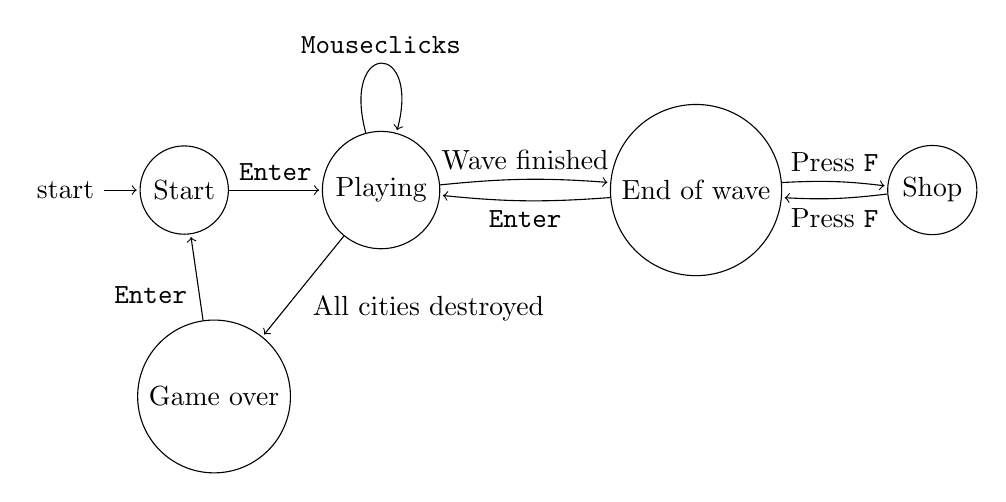
\begin{tikzpicture}[shorten >=1pt,node distance=3cm,on grid,auto]
		\node[state,initial] (Start) {Start};
		\node[state] (Playing) [right=of Start, xshift=-0.5cm] {Playing};
		\node[state] (EndOfWave) [right=of Playing, xshift=1cm] {End of wave};
		\node[state] (Shop) [right=of EndOfWave] {Shop};
		\node[state] (GameOver) [below left=of Playing, yshift=-0.5cm] {Game over};
		
		\path[->]
		(Start) edge node {\texttt{Enter}} (Playing)
		(Playing) edge [loop above] node {\texttt{Mouseclicks}} (Playing)
				  edge[above, bend left=5] node {Wave finished} (EndOfWave)
				  edge node {All cities destroyed} (GameOver)
		(EndOfWave) edge[below, bend left=5] node {\texttt{Enter}} (Playing)
					edge[above, bend left=5] node {Press \texttt{F}} (Shop)
		(Shop) edge[below, bend left=5] node {Press \texttt{F}} (EndOfWave)
		(GameOver) edge node {\texttt{Enter}} (Start);
					
\end{tikzpicture}
\caption{State machine of the game.}
\end{figure}
\noindent
The idea is that on each \texttt{update()} or \texttt{handleInput()} step, the current state will return what the next state should be. For example if the game is currently in the \texttt{EndOfWaveState} and it gets the enter key - the key to start the next wave - it returns a \texttt{PlayingState} with the next wave of enemies. This allows each state to only keep track of themselves and handle everything that happens in the state within their own class. The controller then does not care about what each state is or what it does, but simply calls the update and draw functions of the current state.
\n
To complement the state machine, there are three classes that encapsulate many game properties. The \texttt{GameContext} class is used to encapsulate all information about the game, such as the lists of objects, the physics engine, the current level etc. \texttt{GameInfo} is for all information that is displayed to the player, for example the number of missiles left or the score. \texttt{GameInput} represents all the input from the player and has fields such as the mouse position and the key that was pressed.


\section{Conclusion}

\printbibliography

\end{document}